% !TeX root = neura_v1.tex
% !TeX program = latexmk
\documentclass[5p,times]{elsarticle}

\usepackage[T1]{fontenc}
\usepackage[utf8]{inputenc}
\usepackage{microtype}
\usepackage{amsmath,amssymb}
\usepackage{amsthm}
\usepackage{array}
\usepackage{booktabs}
\usepackage{graphicx}
\usepackage{algorithm}
\usepackage{algpseudocode}
\usepackage{pgfplots}
\usepackage{pgfplotstable}
\usepackage{xcolor}
\usepackage[hyphens]{url}
\usetikzlibrary{positioning,arrows.meta,shapes.geometric,calc}
\usepgfplotslibrary{groupplots}
\usepackage[colorlinks=true,linkcolor=blue,citecolor=blue,urlcolor=blue]{hyperref}

\pgfplotsset{compat=1.18}
\usepackage{tabularx}
\usepackage{booktabs}
\newcolumntype{Y}{>{\raggedright\arraybackslash}X}
\newtheorem{proposition}{Proposition}
\newtheorem{corollary}{Corollary}

\definecolor{SNNBlue}{RGB}{31,119,180}
\definecolor{TEOrange}{RGB}{255,127,14}
\definecolor{ECMPGreen}{RGB}{44,160,44}
\definecolor{BanditRed}{RGB}{214,39,40}
\definecolor{BaselineGray}{RGB}{120,120,120}
\definecolor{MemoryPurple}{RGB}{148,103,189}
\definecolor{FullTeal}{RGB}{23,190,207}

\journal{Computer Networks}
\biboptions{numbers,sort&compress}
\emergencystretch=3em

\pgfplotsset{
ieeeplot/.style={
width=\columnwidth,
height=0.68\columnwidth,
tick label style={font=\footnotesize},
label style={font=\footnotesize},
legend style={font=\footnotesize, draw=none, fill=none},
title style={font=\footnotesize},
grid=both,
major grid style={draw=black!12},
minor grid style={draw=black!6},
ymajorgrids=true,
xmajorgrids=false,
line width=0.95pt,
mark size=2.2pt,
},
ieeebar/.style={
ybar,
bar width=8pt,
enlarge x limits=0.18,
nodes near coords={\pgfmathprintnumber[fixed,precision=2]{\pgfplotspointmeta}},
every node near coord/.append style={font=\scriptsize, rotate=90, anchor=west, /pgf/number format/fixed},
},
}

\begin{document}
\emergencystretch=2em
\begin{frontmatter}

\title{NEURA: Local Excitable Routing Control for Stress-Adaptive Networks}



\author[zky]{Haoming Guo}
\author[xidian]{Zhiyuan Ren\corref{cor1}}
\ead{zyren@xidian.edu.cn}
\author[xidian]{Yuehan Li}
\author[xidian]{Wenchi Cheng}
\address[zky]{Institute of Software, Chinese Academy of Sciences, 4 South Fourth Street, Zhong Guan Cun, Beijing 100190, China}
\address[xidian]{School of Telecommunications Engineering, Xidian University, Xi'an 710071, China}
\cortext[cor1]{Corresponding author}
\tnotetext[t1]{This work was supported by the National Key Research and Development Program of China (No. 2024YFE0200300).}

\begin{abstract}
Severe localized stress can create routing-control amplification: a local queueing or impairment event is converted into widespread control dissemination, repeated forwarding-state rewrites, and recovery-period churn. This paper studies how routing adaptation can be governed as a local, sparse, and recovery-aware control process. We introduce NEURA, a white-box local excitable routing-control law that combines local accumulation, thresholded sparse advertisements, refractory suppression, short-term memory, and guarded switching. Mechanism-level analysis bounds per-candidate firing frequency and gives a sufficient condition under which attenuated perturbations locally extinguish below the decay margin. Discrete-event simulations and packet-level ns-3 validation evaluate NEURA against periodic traffic engineering, triggered traffic engineering, multipath routing, and lightweight learning-based routing under hotspot and repeated-disturbance workloads, with gray-failure and sensitivity checks in the supplementary material. In the tested settings, NEURA occupies a low-control and low-churn operating point while preserving high usable delivery; for example, at a representative 3$\times$ hotspot workload, NEURA achieves $93.6\%$ burst-window delivery with $9.51$ MB of control traffic, compared with $97.3\%$ and $59.6$ MB for OSPF-TE. The results show that routing adaptation can be shaped to limit the spatial and temporal amplification of control activity under stress.
\end{abstract}

\begin{keyword}
routing-control amplification \sep local excitable control \sep stress-adaptive routing \sep event-driven control plane \sep control overhead \sep route churn
\end{keyword}

\end{frontmatter}

\section{Introduction}

Modern routing systems are expected to react quickly to localized failures, congestion bursts, and non-binary impairments. Under severe stress, however, the cost of adaptation can become part of the disturbance. A local hotspot may trigger widespread control dissemination, repeated forwarding-state rewrites, and recovery-period oscillations long after the original pressure has begun to weaken. This paper refers to this phenomenon as routing-control amplification: the data-plane disturbance is local, but the routing adaptation it induces can become spatially broad, temporally dense, and operationally expensive.

Routing-control amplification is especially problematic in stress-adaptive and emergency-style networks. Degradation in these networks is often localized, recurrent, and operationally urgent, while global coordination may be delayed, unavailable, or too costly to invoke for every short-lived shock. In battery-powered field systems and CPU-constrained edge routers, control expansion can consume energy, interrupt scarce local processing time, and increase the amount of forwarding state that must be rewritten during an incident. The design problem is therefore not only how to preserve useful delivery under stress, but how to keep the routing response itself local, sparse, and recovery aware.

Existing routing approaches offer important pieces of this broader problem. Periodic traffic engineering methods can preserve strong service quality through frequent dissemination and recomputation. Multipath routing improves load spreading through path diversity. Learning-based adaptive routing can sustain service under changing conditions with expressive online policies. Operational protocols also contain stabilizing devices such as hold-down behavior, throttled advertisements, minimum advertisement intervals, and route-flap damping. These mechanisms reveal the importance of stabilizing routing dynamics, but most routing designs still treat the spatial spread and temporal density of control activity as secondary effects rather than first-class variables of the routing law.

This work takes a different view: routing adaptation under localized stress should be governed as a local excitable control process. In such a process, weak perturbations decay without triggering broad control activity; sufficiently strong local stress can excite a sparse routing response; immediately repeated excitations are suppressed; and recent degradation leaves a short recovery trace that discourages rebound switching. The resulting scientific question is: under localized network stress, how can a routing system preserve usable delivery without converting local disturbances into network-wide control activity and persistent route churn?

NEURA answers this question with a white-box local excitable routing-control law. Its design vocabulary is drawn from neural local dynamics, but the resulting object is an explicit protocol-level control law. Local integration accumulates route perturbations and stress evidence. Threshold activation emits sparse route-quality advertisements. Refractory suppression limits update bursts after firing. Short-term memory preserves recent degradation during recovery. Guarded switching prevents pressure release from immediately becoming next-hop oscillation. NEURA is therefore not designed to find better paths more aggressively; it is designed to make routing adaptation itself temporally sparse and recovery aware.

This operating point changes the interpretation of performance under stress. A routing method that maximizes short-window delivery by continuously rewriting forwarding state may be attractive in well-powered infrastructure networks, while emergency, tactical, edge, or intermittently connected settings place more value on low control traffic and low route churn. In the workloads studied here, NEURA demonstrates that high usable delivery can be maintained with far less measured control-law traffic and substantially fewer route rewrites when the adaptation process is governed by local accumulation, thresholded activation, suppression, memory, and guarded switching.

The contribution is not that any single primitive, such as a threshold, hold-off timer, memory trace, or switching guard, is new in isolation. These mechanisms all have engineering analogues. The contribution is to make routing-control amplification itself the design object: control spread, temporal update density, recovery churn, and usable delivery are treated together and implemented through a single analyzable and reproducible local control law.

The main contributions of this work are summarized as follows.
\begin{enumerate}
\item A routing-control amplification perspective is formulated for stress-adaptive networks. The paper treats control dissemination, route churn, recovery rebound, and spatial blast radius as central system variables induced by localized stress, alongside conventional service metrics.
\item NEURA is introduced as a local excitable routing-control law. The law composes route viability scoring, dual-timescale local accumulation, thresholded sparse triggering, refractory suppression, short-term memory, and guarded switching into an explicit distance-vector-like control layer for localized stress response.
\item The resulting operating point is characterized analytically and experimentally. Mechanism-level analysis gives per-candidate update-rate bounds and a perturbation attenuation condition, while simulations and packet-level ns-3 validation show that NEURA can preserve useful delivery with substantially lower control activity and route churn than representative periodic, event-driven, multipath, and lightweight learning-based baselines.
\end{enumerate}

The remainder of this paper is organized as follows. Section 2 reviews related work. Section 3 formulates routing-control amplification. Section 4 specifies NEURA. Section 5 describes the evaluation methodology. Section 6 reports the core results. Section 7 discusses scope, and Section 8 concludes the paper.

\section{Related Work}

Existing studies on adaptive routing and distributed network control can be broadly organized according to their primary optimization objective and their resulting control behavior under stress. The most relevant prior work falls into four lines: classical link-state and traffic engineering routing, multipath and load spreading routing, learning-based and queue-aware adaptive routing, and brain-inspired or bio-inspired distributed control. These lines provide strong mechanisms for path computation, load spreading, online adaptation, and decentralized control. NEURA addresses a complementary question: how to preserve useful forwarding while keeping the control response to localized stress spatially contained, temporally sparse, and stable during recovery.

\subsection{Classical Link State and Traffic Engineering Routing}

Classical shortest path and link state routing remain the foundation of modern packet networks, with Dijkstra style path computation and OSPF style information dissemination forming the core of many deployed systems \cite{dijkstra1959note,moy1998ospf}. Traffic engineering extensions further enriched this framework by incorporating additional link attributes and by enabling explicit weight optimization for improved utilization and policy control \cite{katz2003ospfte,fortz2000ospfweights,fortz2002changingworld}. More recent traffic engineering frameworks, including segment routing based traffic engineering, service function chain routing, and deterministic network routing-scheduling co-design, have expanded the flexibility of path steering, centralized resource allocation, and constrained path computation \cite{wu2023srte,wang2025rs4sr,liu2024lpulse,zheng2024tsn,wang2025wtsn}. These approaches are highly effective when the dominant objective is path quality, utilization efficiency, delay guarantee, or global engineering performance. NEURA addresses the complementary objective of keeping stress-induced control activity sparse and local under repeated localized disturbances.

The engineering tradition also includes important mechanisms for suppressing unstable control behavior. Examples include path-vector loop-avoidance and route advertisement control in BGP, route flap damping for persistent instability, and diffusing-update mechanisms for loop-free distance-vector convergence \cite{rekhter2006bgp4,villamizar1998rfd,garcialuna1989dual}. NEURA builds on this engineering intuition by organizing hold-off intervals, thresholded emission, memory, and guarded switching around sparse, spatially local, and recovery-aware stress response. This framing also motivates Triggered-TE as the nearest event-driven engineering comparison in the evaluation.

\subsection{Multipath and Load Spreading Routing}

Multipath forwarding provides a practical mechanism for distributing traffic across multiple next hops and remains a strong engineering approach to hotspot mitigation and load spreading \cite{hopps2000ecmp}. Equal cost multipath forwarding is particularly attractive because path diversity can be exploited without requiring entirely new routing semantics. Recent routing studies have also revisited multipath and mobile-sink style path adaptation for resource constrained wireless and sensor networks, where delivery, energy, and mobility interact strongly \cite{singh2025energyaware}. The principal benefit of this line of work lies in improved forwarding flexibility and reduced concentration of load on a single transit region. NEURA treats the quietness and locality of adaptation as explicit objectives alongside useful delivery, making multipath methods strong service oriented baselines in the present study.

\subsection{Learning Based and Queue Aware Adaptive Routing}

Adaptive routing has long been studied from a learning perspective. Early reinforcement learning based schemes such as Q routing and predictive Q routing demonstrated that route selection could be improved through online experience under changing network conditions \cite{boyan1993qrouting,choi1995pqrouting}. More recent work has extended this direction through deep reinforcement learning, graph neural networks, and hybrid intelligent networking frameworks \cite{schulman2017ppo,you2019multiagentdrl,almasan2019drlgnn,jiang2024gnn,tam2024survey}. Representative recent studies address DRL-assisted SDN traffic engineering, topology-generalizable GNN and DRL routing, multi-agent traffic engineering, resilient routing for LEO mega-constellations, distributed intelligent traffic engineering, and GNN-based network performance modeling \cite{pei2024efficientte,ding2024grom,guo2024mate,zhang2025scair,bai2025grlrr,ai2025topog,guo2025dite,ferriol2023routenetfermi,he2024causalgnn,zhang2023tbppo}. These methods improve service performance and optimization capability under dynamic conditions. NEURA targets a different control object: the dynamics of the adaptation process itself, including update density, blast radius, and recovery churn.

A related but distinct line of work is represented by queue aware and backpressure style control, in which local queue states are used to drive distributed scheduling and routing decisions with strong stability properties \cite{tassiulas1992stability,neely2010stochastic}. This literature establishes the importance of pressure driven local control in networking. NEURA shares this use of local stress signals and applies it to a low-control and low-churn routing operating point in which localized overhead is treated as a primary design objective.

\subsection{Brain Inspired and Bio Inspired Distributed Control}

Biologically inspired networking has been extensively explored as a source of distributed adaptation, self organization, and resilience in complex networked systems \cite{dressler2010survey,meisel2010taxonomy}. Representative examples include ant based routing, pheromone style reinforcement, and other nature inspired search and adaptation mechanisms for mobile and tactical environments \cite{dicaro1998antnet,dicaro2005anthocnet,ducatelle2006anthocnetanalysis}. Cognitive packet networking further extended this direction by allowing packets and nodes to participate in online route adaptation through embedded decision making and learning \cite{gelenbe2000cognitivepackets,gelenbe2001design,gelenbe2001measurement,ray2022cpn}. In most of these studies, however, the biological or cognitive viewpoint is used primarily as a source of decentralized heuristics, exploratory behavior, or adaptive metaphors.

NEURA uses this line of work as a source of local-dynamics primitives for routing control. In spiking neural dynamics, local accumulation, thresholded response, and transient suppression are treated as explicit computational primitives \cite{maass1997thirdgen,gerstner2002spiking,auge2021encoding,han2021snnsurvey}. NEURA translates these primitives into four protocol functions needed for stress-adaptive routing: accumulating local disturbance evidence, emitting sparse updates, suppressing immediate retriggering, and retaining temporary recovery hysteresis. From this perspective, NEURA is a white box local excitable routing-control law for localized, sparse, and recovery aware distributed adaptation under severe network stress.

NEURA does not replace global traffic engineering, ECMP-style throughput optimization, or learning-based policy search. Its role is narrower: it provides an explicit local control semantics for stress-induced amplification, with mechanisms that can be inspected, bounded at the candidate level, and attributed experimentally.

\section{Problem Formulation}

\subsection{Network Model}

The communication system is modeled as a time varying graph
\begin{equation}
G(t) = (V, E(t)),
\end{equation}
where $V$ is the node set and $E(t)$ is the directed link set active at time $t$. Each directed link $(u,v) \in E(t)$ is associated with an effective transmission cost
\begin{equation}
c_{uv}(t) = c^{\mathrm{base}}_{uv} + c^{\mathrm{dyn}}_{uv}(t),
\end{equation}
where $c^{\mathrm{base}}_{uv}$ denotes the baseline structural or administrative cost of the link, and $c^{\mathrm{dyn}}_{uv}(t)$ captures transient fluctuations in operating conditions, including localized congestion, variable queueing delay, and physical link degradation over time.

Each node $u \in V$ observes a localized stress signal $p_u(t)$ defined over time. This state variable represents the immediate resource utilization and physical operating condition at the node, including queue occupancy and burst driven transit delay. In the stress adaptive setting studied here, $p_u(t)$ serves as the primary local stimulus for route adaptation and allows the control plane to react to localized degradation without relying on continuous global dissemination.

For each source destination pair $(u,d)$ with $u \neq d$, the distributed routing mechanism selects a forwarding next hop from the neighbor set $N(u,t)$. The time varying forwarding state is denoted by
\begin{equation}
F_u(d,t) \in N(u,t) \cup \{\varnothing\},
\end{equation}
where $\varnothing$ denotes the absence of a usable next hop. The objective of this routing abstraction is to preserve resilient forwarding and rapid disturbance response, so that packet delivery can continue even when global shortest path guarantees are temporarily degraded.

The path formation substrate is distance-vector-like. Each node evaluates candidate next hops using route quality advertised by neighbors together with local edge cost, stress, memory, and validity state. NEURA contributes the control law that governs when distance-vector-style route-quality changes are accumulated, advertised, suppressed, remembered, and converted into guarded next-hop changes. In this sense, NEURA acts as a control-law layer over a distance-vector-like routing substrate.

\subsection{Objectives and Problem Statement}

The routing control law is evaluated against three objectives, namely service continuity under localized stress, stable recovery after repeated disturbance, and bounded control activity.

For service continuity, the first objective is to maintain a high fraction of reachable source destination pairs throughout the disturbance process. Let $\mathcal{P}$ denote the set of ordered source destination pairs. The reachability ratio at time $t$ is defined as
\begin{equation}
R(t) = \frac{1}{|\mathcal{P}|}\sum_{(u,d)\in\mathcal{P}} \mathbf{1}\{\text{$d$ is reachable from $u$ under }F(t)\},
\end{equation}
where $\mathbf{1}\{\cdot\}$ is the indicator function. This objective also includes hotspot window delivery and bounded path inflation, because useful service under stress cannot be reduced to binary reachability alone.

For recovery stability, the objective is to redirect traffic away from overloaded transit regions without turning disturbance relief into prolonged rebound. This property is evaluated through route churn, service loss duration, and post disturbance recovery behavior.
The cumulative forwarding state rewrite burden is therefore tracked as
\begin{equation}
C_{\mathrm{tot}} = \sum_t \sum_{u\in V}\sum_{d\neq u}
\mathbf{1}\{F_u(d,t)\neq F_u(d,t^-)\},
\end{equation}
where $t^-$ denotes the most recent observation instant before $t$. This quantity captures the route churn that would translate into forwarding table rewrites in a deployed implementation.

For bounded control activity, let $U(t)$ denote the aggregate number of control updates emitted across the network at time $t$. Both the cumulative update burden
\begin{equation}
U_{\mathrm{tot}} = \sum_t U(t)
\end{equation}
and the peak update intensity
\begin{equation}
U_{\mathrm{peak}} = \max_t U(t)
\end{equation}
are monitored. These quantities characterize whether localized stress remains confined to a sparse control response or expands into network wide control activity.
When a stressed region $\mathcal{H}$ is known for an evaluation workload, the spatial containment of updates is measured by the hop distance distribution
\begin{equation}
\pi_k = \frac{\sum_t \sum_{u:\mathrm{dist}(u,\mathcal{H})=k} U_u(t)}
{\sum_t \sum_{u\in V} U_u(t)},
\end{equation}
where $U_u(t)$ is the number of updates emitted by node $u$ at time $t$. This distribution is used to quantify the blast radius of control activity around the disturbed region.

The design problem is therefore to construct a distributed routing control law that keeps $U_{\mathrm{tot}}$, $U_{\mathrm{peak}}$, $C_{\mathrm{tot}}$, and the far-distance mass of $\pi_k$ low while preserving useful delivery, reachability, and bounded path inflation under localized stress. In the present work, this problem is addressed by treating routing adaptation as a local excitable process, and NEURA is developed as its routing instantiation through local accumulation, thresholded activation, transient suppression, and short term memory.

\section{Local Excitable Construction and NEURA Control Law}

In this section, the local excitable construction is specified and the resulting NEURA control law is defined. A small set of local dynamics primitives is used as a structured basis for protocol construction under severe localized stress. Through this construction, localized activation, bounded propagation, transient suppression, and recovery aware adaptation are jointly encoded into a white box routing control law.

\subsection{Primitive to Protocol Mapping}

\begin{figure*}[htbp]
\centering
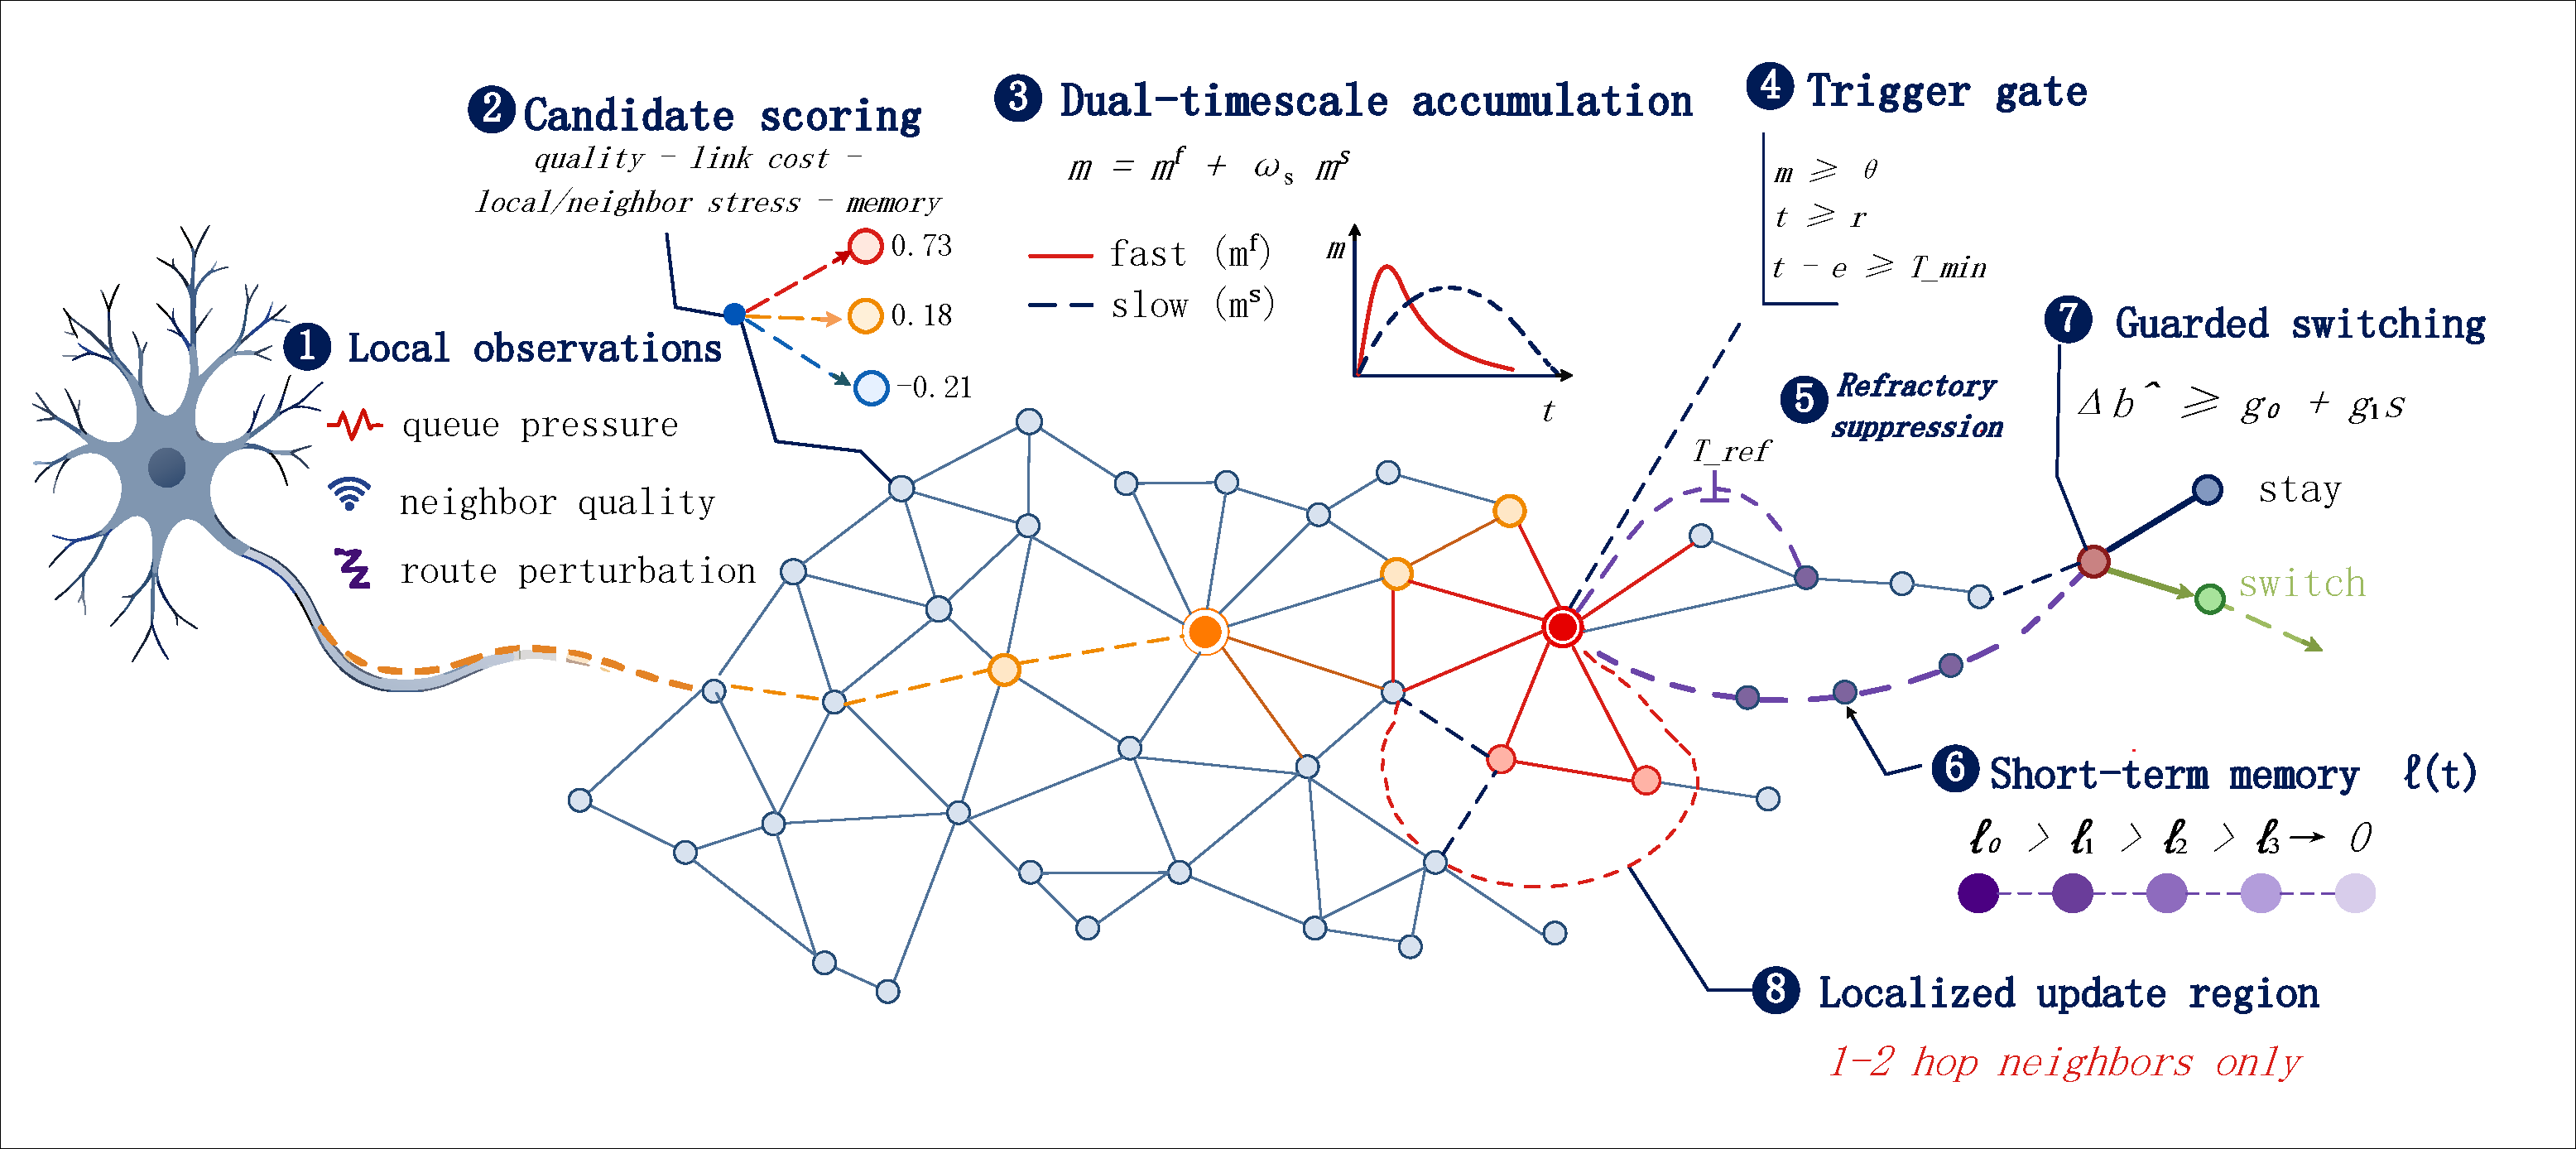
\includegraphics[width=1.0\textwidth]{figures/neura-method-with-tref.pdf}
\caption{Local excitable construction in NEURA. Neural local dynamics primitives, namely integration, threshold activation, refractory suppression, and short term memory, are translated into routing control semantics including local accumulation, sparse triggering, burst suppression, and recovery hysteresis. The resulting control behavior targets localized, sparse, and recovery aware adaptation, with hop bounded propagation and guarded switching under stress.}
\label{fig:method}
\end{figure*}

The central design step of NEURA is a mapping from neural local dynamics primitives to distributed routing control semantics, as summarized in Fig.~\ref{fig:method}. The mapping specifies a local excitable routing process using explicit state variables and triggering rules.

As illustrated in Fig.~\ref{fig:method}, four local dynamics primitives are retained. First, integration is mapped to the accumulation of route perturbations and local stress over time. Through this mapping, routing control is not triggered by a single instantaneous fluctuation alone, but by the local buildup of disturbance evidence. Second, threshold activation is mapped to sparse update triggering. A control update is therefore emitted only when the accumulated local state exceeds a prescribed activation condition. Third, refractory behavior is mapped to transient suppression. Once a control action has been triggered, immediate retriggering is inhibited for a bounded interval, so that repeated local oscillations are not translated into bursty control activity. Fourth, short term memory is mapped to recovery hysteresis. Recently stressed directions remain temporarily less attractive even after the disturbance begins to weaken, so that rebound and excessive switching can be suppressed during recovery.

This mapping defines the construction vocabulary of NEURA. As also indicated in Fig.~\ref{fig:method}, the resulting routing behavior is characterized by localized activation, bounded propagation, and guarded switching under stress. Route adaptation is governed by explicit local state evolution, thresholded activation, temporary suppression, and memory mediated recovery, which together form a local excitable control law.

Each primitive in the mapping has a natural engineering analogue, including integration, thresholds, hold-off timers, memory, and switching guards. NEURA composes these primitives as a distance-vector-like routing-control layer whose target is localized stress management and low control burden. The attribution and sensitivity experiments later explain how this composition shapes burst containment, recovery rebound, and route churn.

At one control epoch, a node observes local queue pressure, refreshes candidate route scores from accepted neighbor advertisements, updates fast and slow trigger states, applies guarded switching to decide whether the forwarding next hop should change, and coalesces pending activations into at most one advertisement per destination. The equations below specify these local steps.

\subsection{Candidate State}

For each node $u$, destination $d \neq u$, and candidate next hop $n$, NEURA maintains the candidate state
\begin{equation}
\mathcal{S}_{u,d,n}(t) =
\left(
\begin{aligned}
&b_{u,d,n}(t),\; m^f_{u,d,n}(t),\; m^s_{u,d,n}(t),\\
&\ell_{u,d,n}(t),\; r_{u,d,n}(t),\; e_{u,d,n}(t),\; \nu_{u,d,n}(t)
\end{aligned}
\right),
\end{equation}
where $b_{u,d,n}(t)$ denotes the route viability score, $m^f_{u,d,n}(t)$ and $m^s_{u,d,n}(t)$ denote the fast and slow accumulation states that govern transmission decisions, $\ell_{u,d,n}(t)$ denotes the short term memory state, $r_{u,d,n}(t)$ denotes the hold off expiration time, $e_{u,d,n}(t)$ denotes the most recent update transmission time, and $\nu_{u,d,n}(t)$ denotes the latest accepted version sequence number.

The combined accumulation state is defined as
\begin{equation}
m(t) = m^{f}(t) + \omega_s m^{s}(t),
\end{equation}
where the $(u,d,n)$ subscripts are omitted for brevity, $m^{f}(t)$ denotes the fast accumulation component, $m^{s}(t)$ denotes the slow accumulation component, and $\omega_s$ denotes the slow timescale weight. Through this decomposition, rapid local reaction and slower recovery sensitive adaptation can be represented within the same control state.

\subsection{Route Viability Calculation}

When node $u$ receives an incremental route update for destination $d$ from neighbor $n$, the candidate route viability score is recalculated by combining downstream route information, local link cost, local stress, neighbor stress, optional incident damage input, and short term memory:
\begin{equation}\label{eq:viability}
\begin{aligned}
b_{u,d,n}(t) ={}& Q_{n,d}(t) - w_c c_{u,n}(t) - w_p p_u(t)\\
&- w_n p_n(t) - w_x x_u(t) - w_\ell \ell_{u,d,n}(t),
\end{aligned}
\end{equation}
where $Q_{n,d}(t)$ denotes the downstream route quality advertised by neighbor $n$, $c_{u,n}(t)$ denotes the local edge cost, $p_u(t)$ and $p_n(t)$ denote the local and neighbor stress signals, $x_u(t)$ denotes an optional incident damage input, and $w_c$, $w_p$, $w_n$, $w_x$, and $w_\ell$ are positive weighting coefficients. In NEURA, $Q_{n,d}(t)$ corresponds to the currently selected downstream route quality toward destination $d$ at node $n$ after local filtering and validity checks. The terms $c_{u,n}(t)$, $p_n(t)$, and $\ell_{u,d,n}(t)$ can change the ordering among candidate neighbors. The terms $p_u(t)$ and $x_u(t)$ are common to all candidates for the same node and destination; they lower the node's advertised route quality, feed the trigger accumulators, and make local stress visible to downstream control decisions. In the hotspot, continuous chaos, and gray failure experiments reported here, $x_u(t)$ is set to zero, and all compared methods react to the same queue derived stress signal.

The raw best candidate is first obtained as
\begin{equation}\label{eq:raw-candidate}
n^{\mathrm{raw}}_{u,d}(t) = \arg\max_{n \in N(u,t)} b_{u,d,n}(t),
\end{equation}
subject to local reachability and validity constraints. This raw candidate is used for local comparison before guarded switching. The advertised route quality corresponds to the currently accepted route after guarded switching, unless a deployment explicitly introduces a separate tentative-candidate signal. The installed forwarding state $F_u(d,t)$ is updated by the guarded switching rule in Section~\ref{sec:guarded-switching}, so that a momentary score advantage does not automatically rewrite the forwarding table.

\subsection{Dual Timescale Accumulation}

NEURA uses local accumulation and decay to determine when route perturbations should trigger control updates. The fast accumulation state integrates recent route perturbation and local stress according to
\begin{equation}\label{eq:fast-accum}
\begin{aligned}
m^{f}_{u,d,n}(t+1) = \max \Big(&0,\,
m^{f}_{u,d,n}(t) - \lambda_f\\
&+ \alpha \Delta b_{u,d,n}(t)
+ \beta p_u(t)
+ \gamma x_u(t)\Big),
\end{aligned}
\end{equation}
where $\lambda_f$ denotes the fast decay factor, $\Delta b_{u,d,n}(t)\ge 0$ denotes the nonnegative magnitude of an externally injected route-quality perturbation, and $x_u(t)$ denotes an optional local incident damage input. In the implementation, $\Delta b_{u,d,n}(t)$ is computed from candidate viability changes caused by local observations or accepted neighbor updates, and can be restricted to degradation-only changes in deployments that only want to trigger on worsening routes. Passive decay of memory, trigger accumulators, and guarded-switching internal state is not treated as a new perturbation injection. A quiescent route state therefore has $\Delta b_{u,d,n}(t)=0$. In the main hotspot, continuous chaos, and gray failure workloads studied in this paper, $x_u(t)$ is set to zero.

The slow accumulation state captures persistent stress and longer lived disturbance effects according to
\begin{equation}\label{eq:slow-accum}
\begin{aligned}
m^{s}_{u,d,n}(t+1) = \max \Big(&0,\,
\rho_s m^{s}_{u,d,n}(t)\\
&+ \beta_s p_u(t)
+ \gamma_s x_u(t)
- \lambda_s\Big),
\end{aligned}
\end{equation}
where $\rho_s$ denotes the slow state retention factor and $\lambda_s$ denotes the slow decay factor.

The combined accumulation state is then given by
\begin{equation}\label{eq:combined-accum}
m_{u,d,n}(t+1) = m^{f}_{u,d,n}(t+1) + \omega_s m^{s}_{u,d,n}(t+1).
\end{equation}
Through this dual timescale construction, rapid local reaction to emerging stress and slower recovery sensitive adaptation under repeated disturbance can be represented within a unified control state.

\subsection{Thresholded Update Triggering}

A candidate route state triggers update transmission when its accumulation state exceeds a prescribed threshold and two temporal rate limiting conditions are satisfied:
\begin{align}
\label{eq:trigger-threshold}
m_{u,d,n}(t) &\geq \theta, \\
\label{eq:trigger-refractory}
t &\geq r_{u,d,n}(t), \\
\label{eq:trigger-mingap}
t - e_{u,d,n}(t) &\geq T_{\min},
\end{align}
where $\theta$ denotes the triggering threshold and $T_{\min}$ denotes the minimum inter transmission interval.

When a candidate is activated, node $u$ marks destination $d$ as pending for advertisement rather than immediately emitting a route update. Candidate activation is therefore a local trigger for re-evaluating the accepted route to destination $d$. After guarded switching has installed or retained the forwarding state, pending activations for the same $(u,d)$ are coalesced into at most one incremental update carrying the currently accepted route quality and installed next-hop context. The emitted message contains the destination identifier, the selected route cost or route quality, the selected next hop context, a version sequence value, a hop bounded lifetime, and the current local stress level. This sparse event driven update mechanism is central to the low overhead operating mode of NEURA.

NEURA is implemented as a local control layer over versioned route-quality advertisements. Accepted updates must pass destination-validity, neighbor-reachability, sequence-freshness, and finite-lifetime checks before affecting candidate scoring or next-hop installation. Guarded switching further requires a stress-dependent advantage over the incumbent route before forwarding state is rewritten. These rules keep stale advertisements and weak transient alternatives from dominating local decisions. The formal analysis below focuses on the control-law properties directly enforced by NEURA, namely bounded update frequency and perturbation attenuation, while the evaluation reports reachability, loop, blackhole, and complete-route indicators for the tested workloads.

\subsection{Transient Suppression}

After activation, the candidate enters a refractory window:
\begin{equation}\label{eq:refractory-update}
r_{u,d,n}(t^+) = t + T_{\mathrm{ref}},
\end{equation}
where $T_{\mathrm{ref}}$ denotes the hold off duration. This transient suppression state prevents immediate retriggering under weak local oscillations and supplies the per-candidate rate limiting used in the mechanism-level bound below.

\subsection{Short Term Memory}

NEURA also maintains a short term memory variable that stores an exponentially decaying trace of recent stress and optional incident damage input:
\begin{equation}\label{eq:memory}
\ell_{u,d,n}(t+1) =
\eta \ell_{u,d,n}(t) + \mu_p p_u(t) + \mu_x x_u(t),
\end{equation}
where $\eta \in (0,1)$ denotes the memory retention factor. This term enters the route viability update through the penalty term $w_\ell \ell_{u,d,n}(t)$. Consequently, recently degraded directions remain temporarily less attractive even after the disturbance begins to weaken. This mechanism supports reduced rebound and smoother post disturbance recovery.
The additive term in Eq.~\eqref{eq:memory} records local stress that is initially common across candidates at node $u$. Directional asymmetry is introduced by the guarded-switching update below: a deselected next hop receives an additional memory boost, while a newly selected next hop receives memory relaxation. Thus the memory mechanism combines a local recovery trace with switch-induced directionality.

\subsection{Guarded Switching and Stress Responsive Release}
\label{sec:guarded-switching}

The full NEURA control law also employs guarded switching so that local stress release is not immediately translated into unnecessary next hop oscillation. Let
\begin{equation}
n^\star_{u,d}(t)=F_u(d,t^-)
\end{equation}
denote the currently selected next hop for destination $d$ before the current refresh step. If no valid incumbent exists, $F_u(d,t)$ is initialized with the valid raw candidate in Eq.~\eqref{eq:raw-candidate}. Otherwise, switching from the incumbent is governed by the guarded comparison below. When $n^\star_{u,d}(t)$ exists, the selected direction stress summary is defined as
\begin{equation}\label{eq:selected-stress}
s_{u,d}(t)=p_u(t)+x_u(t)+\ell_{u,d,n^\star}(t)+\omega_s m^s_{u,d,n^\star}(t).
\end{equation}

Based on this quantity, an effective viability is formed for candidate comparison:
\begin{equation}\label{eq:effective-viability}
\tilde{b}_{u,d,n}(t)=
\begin{cases}
b_{u,d,n}(t)-\psi_{\mathrm{sel}} s_{u,d}(t), & n=n^\star_{u,d}(t),\\
b_{u,d,n}(t)+\psi_{\mathrm{rel}} s_{u,d}(t), & n\neq n^\star_{u,d}(t),
\end{cases}
\end{equation}
where $\psi_{\mathrm{sel}}$ denotes the selected path suppression weight and $\psi_{\mathrm{rel}}$ denotes the alternate path release weight. The provisional challenger is then given by
\begin{equation}
\hat{n}_{u,d}(t)=\arg\max_{n \in N(u,t)} \tilde{b}_{u,d,n}(t).
\end{equation}

A switch is accepted only when the challenger clears an explicit guarded margin:
\begin{equation}\label{eq:switch-guard}
\tilde{b}_{u,d,\hat{n}}(t)\ge \tilde{b}_{u,d,n^\star}(t)+g_0+g_1 s_{u,d}(t),
\end{equation}
where $g_0$ denotes the base switch guard and $g_1$ denotes the stress scaled rebound guard. If Eq.~\eqref{eq:switch-guard} is not satisfied, the current next hop is retained even when another candidate is momentarily better.
The release term exposes alternative routes by penalizing the currently stressed direction and lifting challengers in the comparison, while the stress-scaled guard prevents weak alternatives from causing rebound switching. Under high stress, a switch is accepted only when the challenger has a sufficiently clear effective advantage.

When a guarded switch is accepted, secondary state is updated asymmetrically according to
\begin{align}
\ell_{u,d,n^\star}(t^+) &= \ell_{u,d,n^\star}(t) + \delta_{\mathrm{desel}} \max(s_{u,d}(t), 1),\\
m^{f}_{u,d,n^\star}(t^+) &= \max\left(0, m^{f}_{u,d,n^\star}(t) - 0.5\theta\right),\\
\ell_{u,d,\hat{n}}(t^+) &= \max\left(0, \ell_{u,d,\hat{n}}(t) - \delta_{\mathrm{sel}}\right),
\end{align}
where $\delta_{\mathrm{desel}}$ denotes the deselected route memory boost and $\delta_{\mathrm{sel}}$ denotes the new route memory relaxation. These terms are part of the full routing law used in the reported experiments, and they correspond directly to the switch suppression mechanism examined later in the attribution study. Their function is to prevent local stress release from being converted into avoidable rebound bursts of switching activity.

\subsection{Mechanism-Level Properties of NEURA}

This subsection states local consequences of the NEURA update equations. These are mechanism-level properties rather than claims of global optimality or full distance-vector convergence. They explain two behaviors used later to interpret the experiments: a hard per-candidate firing bound, and local extinction of propagated perturbations whose effect falls below the decay margin.

\begin{proposition}[Quiescence and per-candidate firing bound]
\label{prop:quiescent-bound}
Fix a candidate state $(u,d,n)$ and suppose that, from epoch $t_0$ onward, $p_u(t)=0$, $x_u(t)=0$, and no route viability perturbation is injected, i.e., $\Delta b_{u,d,n}(t)=0$. Then the combined trigger state $m_{u,d,n}(t)$ reaches zero in finite time. Moreover, for any interval of $H$ epochs, the number of updates emitted by this candidate is at most
\begin{equation}
1+\left\lfloor \frac{H}{\tau} \right\rfloor,
\qquad
\tau=\max\{T_{\mathrm{ref}},T_{\min}\}.
\end{equation}
Consequently, if at most $M$ candidate states are trigger eligible over the interval, the aggregate emitted updates are bounded by
\begin{equation}
M\left(1+\left\lfloor \frac{H}{\tau} \right\rfloor\right).
\end{equation}
\end{proposition}

\begin{proof}
Under the stated quiescent condition, Eq.~\eqref{eq:fast-accum} gives
\begin{equation}
m^{f}_{u,d,n}(t+1)
\le \max\big(0,m^{f}_{u,d,n}(t)-\lambda_f\big).
\end{equation}
Since $\lambda_f>0$, the fast component becomes zero after at most
$\lceil m^{f}_{u,d,n}(t_0)/\lambda_f\rceil$ epochs. Similarly, Eq.~\eqref{eq:slow-accum} gives
\begin{equation}
m^{s}_{u,d,n}(t+1)
\le \max\big(0,\rho_s m^{s}_{u,d,n}(t)-\lambda_s\big),
\end{equation}
with $0\le \rho_s<1$ and $\lambda_s>0$. While the slow component is positive, repeated substitution yields
\begin{equation}
m^{s}_{u,d,n}(t_0+k)
\le
\rho_s^k m^{s}_{u,d,n}(t_0)
-\lambda_s\frac{1-\rho_s^k}{1-\rho_s}.
\end{equation}
The right hand side is non positive for finite $k$, so $m^s$ also reaches zero in finite time. Equation~\eqref{eq:combined-accum} then implies finite time decay of $m$.

For the firing bound, let $t_i$ and $t_{i+1}$ be two consecutive trigger epochs for the same candidate. After a trigger, Eq.~\eqref{eq:refractory-update} and Eq.~\eqref{eq:trigger-refractory} require $t_{i+1}\ge t_i+T_{\mathrm{ref}}$, while Eq.~\eqref{eq:trigger-mingap} requires $t_{i+1}\ge t_i+T_{\min}$. Hence $t_{i+1}-t_i\ge \tau$. At most one trigger can occur in each length-$\tau$ subinterval, giving the stated per-candidate and aggregate bounds.
\end{proof}

\begin{proposition}[Local extinction of attenuated cascades]
\label{prop:cascade-extinction}
Consider a candidate state outside the directly stressed region over an interval $[t_0,t_0+H]$, so that $p_u(t)=0$ and $x_u(t)=0$ throughout the interval. If there exists a margin $\epsilon>0$ such that every incoming viability perturbation satisfies
\begin{equation}
\alpha \Delta b_{u,d,n}(t)\le \lambda_f-\epsilon,
\qquad t\in[t_0,t_0+H],
\end{equation}
then the fast accumulation component decreases by at least $\epsilon$ whenever it is positive, and the slow component decays as in Proposition~\ref{prop:quiescent-bound}. In particular, after a finite number of epochs depending only on the initial local state and the parameters, this candidate cannot fire unless a new above-margin perturbation or local stress input arrives.
\end{proposition}

\begin{proof}
With $p_u(t)=0$ and $x_u(t)=0$, Eq.~\eqref{eq:fast-accum} becomes
\begin{equation}
m^{f}_{u,d,n}(t+1)
=
\max\big(0,m^{f}_{u,d,n}(t)-\lambda_f+\alpha\Delta b_{u,d,n}(t)\big).
\end{equation}
The assumed margin gives
\begin{equation}
m^{f}_{u,d,n}(t+1)
\le
\max\big(0,m^{f}_{u,d,n}(t)-\epsilon\big),
\end{equation}
so the fast component reaches zero after at most
$\lceil m^{f}_{u,d,n}(t_0)/\epsilon\rceil$ epochs. The slow component receives no local stress injection and therefore decays by the same argument used in Proposition~\ref{prop:quiescent-bound}. Once both components are zero, the combined accumulation in Eq.~\eqref{eq:combined-accum} is below the trigger threshold $\theta>0$. Thus this candidate cannot emit a further update unless a new perturbation exceeds the local decay margin or a new local stress input is injected.
\end{proof}

\begin{corollary}[Interpretation for locality and recovery]
\label{cor:locality-recovery}
NEURA's low control regime follows from a local rather than global optimality argument. Proposition~\ref{prop:quiescent-bound} bounds the temporal density of updates, while Proposition~\ref{prop:cascade-extinction} gives a sufficient condition under which attenuated route perturbations stop propagating. The memory term in Eq.~\eqref{eq:memory} adds recovery hysteresis: after a stressed direction accumulates memory $\ell_0$, its viability remains penalized by $w_\ell\eta^k\ell_0$ after $k$ quiescent epochs. Therefore a recently degraded direction must overcome a decaying but nonzero margin before it becomes attractive again, which explains the rebound suppression and reduced route churn observed in the evaluation.
\end{corollary}

The distance-vector-like substrate also uses versioned advertisements, finite lifetimes, neighbor reachability checks, destination validity checks, and guarded switching before a next hop is installed. These engineering checks are evaluated empirically through reachability, loop, and blackhole indicators; the formal statements above intentionally remain local to the control law.

\subsection{Per Node Update Procedure}

Algorithm~\ref{alg:neura-control-loop} summarizes the per node control loop induced by the preceding equations.

\begin{algorithm}[t]
\caption{NEURA Localized Control Loop at Node $u$}
\label{alg:neura-control-loop}
\begin{algorithmic}[1]
\For{each control epoch $t$}
    \State observe local stress $p_u(t)$ and optional incident damage input $x_u(t)$
    \State receive neighbor incremental updates and refresh candidate set
    \For{each destination $d$ and candidate next hop $n$}
        \State update route viability score $b_{u,d,n}(t)$
        \State update fast and slow accumulation states
        \State update short term memory trace $\ell_{u,d,n}(t)$
        \If{$m_{u,d,n}(t) \ge \theta$ and hold off constraints are satisfied}
            \State mark destination $d$ as pending for advertisement
            \State enter transient suppression interval
        \EndIf
    \EndFor
    \State apply guarded switching to select the forwarding next hop
    \For{each destination $d$ marked pending}
        \State coalesce activations and emit at most one update for the accepted route
    \EndFor
\EndFor
\end{algorithmic}
\end{algorithm}

\subsection{Implemented Parameterization}

Table~\ref{tab:neura-params} lists the default parameter settings retained in the main text. Only the parameters that are referenced directly by the control equations or revisited in the sensitivity and attribution studies are included here.

\begin{table}[t]
\centering
\footnotesize
\caption{Implemented defaults retained in the main text.}
\label{tab:neura-params}
\resizebox{\columnwidth}{!}{%
\begin{tabular}{>{\raggedright\arraybackslash}p{2.4cm}>{\raggedright\arraybackslash}p{0.8cm}>{\raggedright\arraybackslash}p{4.0cm}}
\toprule
Implementation Label & Value & Manuscript Role \\
\midrule
threshold & 1.4 & firing threshold $\theta$ \\
refractory ticks & 4 & refractory duration $T_{\mathrm{ref}}$ \\
minimum emit ticks & 3 & minimum emission interval $T_{\min}$ \\
update TTL & 12 & hop bounded route update lifetime \\
edge weight & 1.0 & local edge cost weight $w_c$ \\
self-pressure weight & 1.0 & local stress weight $w_p$ \\
neighbor-pressure weight & 0.5 & neighbor stress weight $w_n$ \\
memory weight & 0.5 & memory penalty $w_{\ell}$ \\
fast leak & 0.24 & fast decay $\lambda_f$ \\
slow decay & 0.88 & slow state retention $\rho_s$ \\
slow leak & 0.08 & slow decay $\lambda_s$ \\
slow weight & 0.35 & slow timescale weight $\omega_s$ \\
memory decay & 0.78 & memory retention $\eta$ \\
suppression penalty & 0.18 & selected path suppression weight $\psi_{\mathrm{sel}}$ \\
release term & 0.08 & alternate path release weight $\psi_{\mathrm{rel}}$ \\
switch guard & 0.45 & base switch guard $g_0$ \\
rebound guard & 0.35 & stress scaled rebound guard $g_1$ \\
deselected memory boost & 0.55 & deselected route memory boost $\delta_{\mathrm{desel}}$ \\
selected memory relaxation & 0.25 & new route memory relaxation $\delta_{\mathrm{sel}}$ \\
\bottomrule
\end{tabular}
\vspace{1mm}
}
\end{table}

\section{Evaluation Methodology and Setup}

\subsection{Evaluation Philosophy}

NEURA is evaluated in a custom discrete event simulation framework designed to isolate control plane propagation dynamics from lower layer protocol noise. The simulator maintains per node route state, event driven route delta propagation, queue driven local stress, and a common metric extraction pipeline across all compared methods. Each simulation tick represents a nominal $10$ ms control epoch, so that reaction latency and suppression intervals can be reported in both ticks and approximate wall clock time. This level of abstraction is appropriate for studying localized control law behavior while preserving a consistent comparison across routing families.

Packet-level ns-3 validation is added as a complementary evidence path focused on packetized control transmission, DropTail queues, and online queue sampling. It is not a full distributed protocol-stack implementation of NEURA. Instead, it tests whether the operating-point ordering remains visible when control and data traffic are packetized and source host routes are updated from sampled DropTail queue pressure. The main evidence path remains the discrete event routing simulator, which is designed to characterize localized control behavior across the full ER-100 matrix.

This evaluation assumes local observability of adjacent link state. In the simulator, hard adjacency changes enter through the time varying edge set $E(t)$. An optional incident damage signal $x_u(t)$ is available only to endpoints of explicitly failed links and is inactive in the main hotspot, continuous chaos, and gray failure result paths. Those main results are driven by the shared queue derived stress signal. The reported overhead measurements quantify adaptive routing-control payloads under a common accounting model.

\subsection{Topology and Baselines}

The routing dynamics are evaluated primarily on connected Erdos--Renyi random graphs. This topology family provides moderate path diversity without imposing rigid structural bias, which matches the uncertain connectivity patterns often encountered in rapidly deployed communication systems. For each trial, an undirected graph is sampled with node count $N=100$ and edge probability $p=0.06$ until a connected realization is obtained, after which each edge is instantiated as a bidirectional link. To reduce dependence on a single graph family, supporting topology checks are also performed on connected $100$ node Barab\'asi--Albert and random geometric graphs. The random geometric case uses a connection radius of $0.17$, thereby imposing spatially local connectivity and providing a stricter test of whether localized control behavior persists beyond ER style path mixing.

NEURA is compared against four baseline classes that represent distinct control plane paradigms. The first is a classical traffic engineering baseline based on periodic link state dissemination. It incorporates stress sensitive link penalties into path selection and serves as the reference for fixed interval adaptivity. The second is a nearest neighbor engineering baseline based on triggered traffic engineering with thresholded updates, a minimum emission interval, switching hysteresis, and a slower background refresh than OSPF-TE. It provides the closest event-driven engineering comparison for isolating how memory, refractory suppression, and guarded switching shape the dynamics of adaptation. The third is a multipath traffic engineering strategy based on equal cost multipath forwarding, which represents a strong engineering approach to hotspot mitigation through spatial load spreading. Its reported control cost comes from the accompanying TE refresh and multipath state maintenance in the baseline controller. The fourth is a lightweight learning based adaptive method based on bandit routing, which represents online adaptive control without the training complexity of deep reinforcement learning. Together, these methods cover representative control paradigms. To avoid synchronized artifacts, all periodic refresh baselines use node local periodic timers with independent phase offsets. The compared methods and their roles are summarized in Table~\ref{tab:methods}.

Baseline parameters are chosen to represent reasonable operating points on the same delivery-control tradeoff. OSPF-TE, Triggered-TE, TE+ECMP, and Bandit all observe the same queue-derived stress signal where applicable. NEURA parameter sensitivity and additional engineering-knob sweeps are reported in the supplementary material.

\subsection{Workloads and Stress Formulation}

Three core disturbance workloads are used in the main text. The first is a pressure-driven impulse workload, in which a sudden traffic burst is injected over a designated hotspot node in order to measure temporal reaction speed. The second is a closed-loop hotspot avoidance workload, in which source-destination flows traversing a central transit node receive a multiplicative demand increase. The third is a repeated-disturbance workload, in which three hotspot shocks are injected in sequence. Gray-failure, startup, path-stretch, topology-family, attribution, and sensitivity checks are reported in the supplementary material. For each sampled topology, the hotspot is selected as a high-transit node under the initial shortest-path routing state, and source-destination flows are generated over reachable pairs.

The traffic model is discrete in time. Link transmission is bounded by per link service capacity and fixed queue limits, and excess offered load accumulates in local queues. This queue state captures burst driven overload, pressure propagation, and post burst recovery, and it forms the foundational stress signal for both NEURA and the queue sensitive baselines. For node $u$, the local stress signal $p_u(t)$ is defined as the mean normalized queue occupancy of its incident directed links:
\begin{equation}
p_u(t) = \frac{1}{|N(u,t)|} \sum_{v \in N(u,t)} \min \left(1, \frac{q_{u,v}(t)}{Q_{\max}} \right),
\end{equation}
where $q_{u,v}(t)$ denotes the queue occupancy on link $(u,v)$ and $Q_{\max}$ denotes the queue capacity limit. The OSPF-TE, Triggered-TE, and TE+ECMP baselines use the same queue derived signal through the dynamic link cost model
\begin{equation}
c_{u,v}(t) = c^{0}_{u,v} + \kappa \min \left(1, \frac{q_{u,v}(t)}{Q_{\max}} \right),
\end{equation}
where $c^{0}_{u,v}$ denotes the static edge weight and $\kappa$ denotes the congestion cost coefficient. This shared input keeps the comparison aligned at the level of observed network stress while allowing the control mechanisms themselves to differ.

All compared methods exchange fixed format logical control records in the simulator. One emitted update is counted as one common $32$ byte record, so reported bytes equal emitted update count times the shared algorithmic payload size. NEURA's lower byte count therefore reflects fewer and more localized updates under the same per-message budget. The method structure in Table~\ref{tab:methods} separates two sources of overhead reduction: NEURA and Triggered-TE share a DV-like route-quality advertisement substrate, while OSPF-TE and TE+ECMP use link-state TE dissemination. The comparison between NEURA and Triggered-TE therefore isolates the additional effect of the local excitable law, including sparsification, refractory suppression, memory, and guarded switching. Standard link, network, and transport headers are outside this logical-control accounting, and the same definition applies to the control bars in the result figures.

\subsection{Metrics}

The evaluation reports four metric groups. The primary control plane metrics are disturbance window control bytes, control message rate, route change rate, spatial containment of update propagation, startup convergence latency, and service loss duration under repeated disturbances. These quantities characterize how much control activity is generated, how far it spreads, how quickly forwarding state is rewritten, how quickly the routing system becomes usable, and how long useful service remains degraded under sustained shocks.

The secondary service metrics are burst window delivery ratio, burst window loss ratio, burst window mean delay, and service loss duration under repeated disturbances. These metrics verify that low overhead control still produces useful routing adaptation during stress. For the ns-3 validation path, packet delivery, packetized control transmission, route rewrites, post-stress tail switching, and TCP goodput are additionally reported. Supplementary safety and robustness metrics are also collected, including pairwise reachability ratio, loop ratio, blackhole ratio, cumulative emitted updates, and parameter sensitivity, linking the low-overhead operating point to routing-safety indicators.

\begin{table*}[t]
\centering
\small
\caption{Compared methods and their control-plane structure in the study.}
\label{tab:methods}
\setlength{\tabcolsep}{4pt}
\begin{tabularx}{\textwidth}{@{}l p{3.0cm} p{3.2cm} X@{}}
\toprule
Method & Routing substrate & Triggering policy & Stabilization / role \\
\midrule
NEURA & DV-like route-quality ads & Local excitable threshold & Refractory plus memory plus guarded switching \\
OSPF-TE & Link-state SPF & Fixed interval & Periodic recomputation \\
Triggered-TE & DV-like route-quality ads & Thresholded plus slow refresh & Minimum gap plus simple hysteresis plus slow refresh \\
TE+ECMP & Link-state TE plus multipath & Fixed interval & Periodic TE plus multipath state \\
Bandit & Online per-destination policy & Online adaptive & Exploration/exploitation updates \\
\bottomrule
\end{tabularx}
\end{table*}


\section{Evaluation Results}

\subsection{Shock Response Under Local Stress}

The first experiment examines whether a routing law can remain quiet before a localized hotspot, activate when local stress appears, and preserve useful delivery during the same burst window. Figure~\ref{fig:shock-response} aligns control traffic and delivery on a common time axis.

Before the shock, from approximately $300$ to $390$~ms, NEURA remains near $1.1$~KB of control traffic per control epoch. Triggered-TE, OSPF-TE, and Bandit remain near $311$~KB, $378$~KB, and $626$~KB, respectively. NEURA therefore enters the disturbance from a much quieter control state rather than from a continuously active adaptation regime.
This residual pre-shock traffic uses the same fixed-size logical update accounting applied to all methods and corresponds to low-frequency route-quality maintenance and residual local convergence activity within the measured window.

After the hotspot starts at $400$~ms, NEURA rises to about $79$~KB by $450$~ms while restoring delivery from $68.5\%$ at shock onset to $96.7\%$. Triggered-TE reaches similar burst-window delivery, moving from $89.7\%$ to $95.5\%$, but it does so from a pre-shock control level already near $311$~KB. The comparison separates responsiveness from permanent control activity: sparse activation can react quickly without keeping the whole control plane hot before the event.

During the burst window, NEURA averages about $22$ route changes per control epoch, compared with about $12$ for Triggered-TE, $108$ for OSPF-TE, and $3779$ for Bandit. Although Triggered-TE performs slightly fewer route changes in this short window, NEURA keeps churn far below the heavier engineering and learning-based baselines while being coupled to the quietest pre-shock state. The large Bandit churn reflects fine-grained online exploration and per-destination route adaptation under burst pressure in this lightweight learning baseline. TE+ECMP remains in the high-delivery regime in the delivery panel; its broader routing cost is examined in the stress sweep.

The temporal conclusion is that localized stress can be handled without committing the network to a permanently aggressive control schedule. The calm pre-shock period is therefore part of the intended operating behavior of the routing law.

\begin{figure*}[t]
\centering
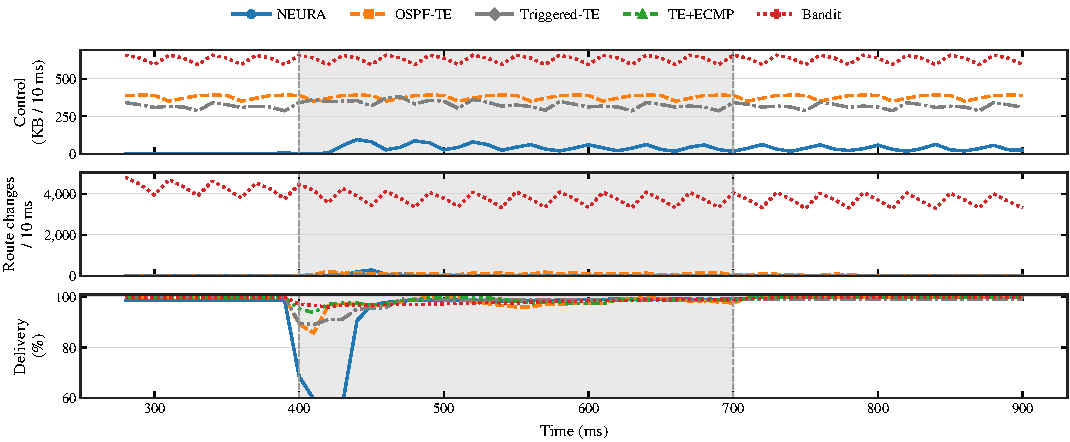
\includegraphics[width=\textwidth]{figures/generated/fig1_shock_response.pdf}
\caption{Shock response under localized stress. The shaded interval marks the burst window. NEURA stays quiet before the shock, reacts only inside the disturbance interval, and keeps route churn far below the engineering and learning baselines.}
\label{fig:shock-response}
\end{figure*}


\subsection{Blast Radius of Control Activity}

The second experiment asks how far a localized shock propagates into the control plane. Figure~\ref{fig:blast-radius} reports the share of hotspot-window updates generated at the hotspot, one hop away, two hops away, and three or more hops away.

On the formal ER-100 matrix, all NEURA hotspot-window updates remain within one hop of the stressed node: about $11.7\%$ are generated at the hotspot and about $88.3\%$ one hop away. In absolute terms, the locality experiment records about $44.6$ NEURA emitted updates under the hotspot window, compared with about $392$ for Triggered-TE and about $420$ for the matched OSPF-TE periodic setting. The nearest event-triggered baseline remains much less localized: only about $17.4\%$ of Triggered-TE updates stay within one hop, while about $49.1\%$ are generated two hops away and about $33.5\%$ at three or more hops. OSPF-TE exhibits a similar multi-hop pattern, with only about $14.0\%$ of its hotspot-window updates within one hop, roughly $48.0\%$ two hops away, and another $38.0\%$ at three or more hops. Thus, NEURA contains the control response around the disturbed region, whereas both the event-triggered engineering baseline and periodic link-state adaptation readily expand into multi-hop control activity.

The same qualitative locality pattern appears in the supporting BA-100 and RGG-100 topology checks reported in the supplementary material. This result supports the structural claim that local stress can be handled without turning every disturbance into network-wide control activity.

\begin{figure}[t]
\centering
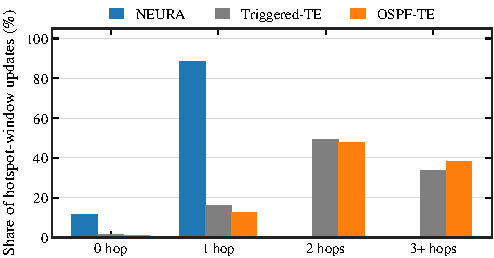
\includegraphics[width=\columnwidth]{figures/generated/fig2_blast_radius.pdf}
\caption{Blast radius of control activity during a localized hotspot event. The bars report the mean update share generated at each hop-distance bucket from the stressed region. NEURA is compared with the nearest event-triggered engineering baseline and the periodic OSPF-TE baseline.}
\label{fig:blast-radius}
\end{figure}


\subsection{Service Preservation and Control Cost Under Increasing Stress}
The third experiment makes the central systems tradeoff explicit by sweeping the hotspot-demand multiplier while keeping link capacities fixed. Fig.~\ref{fig:stress-tradeoff} reports burst-window delivery and control traffic, while route-change totals are summarized in the text.

At the representative $3\times$ hotspot workload, NEURA preserves $93.6\%$ burst-window delivery with $9.51$~MB of control traffic. Triggered-TE preserves $97.4\%$ with $54.2$~MB, OSPF-TE preserves $97.3\%$ with $59.6$~MB, TE+ECMP preserves $98.2\%$ with $115.2$~MB, and Bandit preserves $97.9\%$ with $99.6$~MB. Relative to Triggered-TE and OSPF-TE, NEURA gives up about $3.8$ and $3.7$ percentage points of burst-window delivery, respectively, while reducing logical control traffic by roughly a factor of five to six.

The same stress point exposes the churn tradeoff. NEURA averages about $100$ route changes per node over the full run, compared with about $118$ for Triggered-TE, $172$ for OSPF-TE, $242$ for TE+ECMP, and more than $6380$ for Bandit. At the harsher $5\times$ workload, NEURA preserves $85.8\%$ delivery with $10.6$~MB of control traffic, whereas Triggered-TE preserves $87.2\%$ with $56.7$~MB and OSPF-TE preserves $86.9\%$ with $59.6$~MB. The nearest-neighbor engineering baseline closes much of the service gap, but it still pays a control budget roughly five times larger than NEURA across the representative stress range.

The stress sweep establishes the main systems argument: localized stress can be mitigated without coupling the network to proportionally large and persistent control-plane activity.
\begin{figure}[t]
\centering
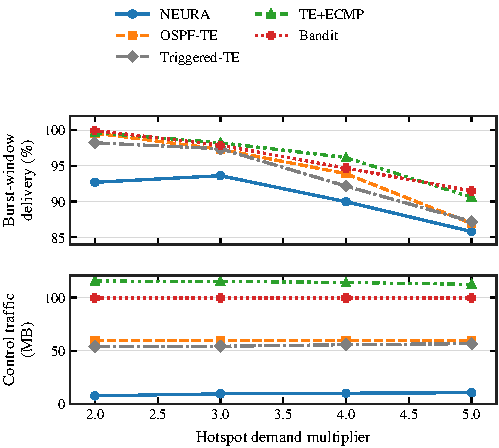
\includegraphics[width=\columnwidth]{figures/generated/fig3_stress_tradeoff.pdf}
\caption{Mitigation cost under increasing stress. The upper panel reports retained service during the hotspot window. The lower panel reports the control traffic required over the same disturbance interval. NEURA accepts a modest delivery penalty while maintaining the lowest control-cost operating point across the stress sweep.}
\label{fig:stress-tradeoff}
\end{figure}


\subsection{Repeated Disturbance and Robustness}

The fourth experiment moves from isolated shocks to sustained volatility. Three hotspot shocks are injected in sequence, and the evaluation asks whether the control plane settles between shocks or drifts into repeated update storms. Fig.~\ref{fig:continuous-chaos} reports the resulting time series and stability indicators.

Over the full sequence, NEURA consumes $9.14$~MB of total control traffic, compared with $52.09$~MB for OSPF-TE, $48.43$~MB for Triggered-TE, $99.85$~MB for TE+ECMP, and $87.01$~MB for Bandit. It also accumulates about $100$ route changes per node, compared with about $210$ for OSPF-TE, $122$ for Triggered-TE, $282$ for TE+ECMP, and $5645$ for Bandit. The service metrics remain close: mean service-loss duration is $7.4$ ticks for NEURA, $7.2$ for OSPF-TE, and $6.8$ for Triggered-TE, while mean burst-window delivery is $96.0\%$, $96.6\%$, and $96.4\%$, respectively. TE+ECMP and Bandit improve these service values further, but at much higher cumulative control and churn cost.

Under sustained volatility, NEURA remains operational and confines total control activity to a much lower level than the baselines, while preserving service close to the traffic-engineering alternatives. Additional startup, path-stretch, gray-failure, topology-family, attribution, and sensitivity results are provided in the supplementary material.
\begin{figure*}[t]
\centering
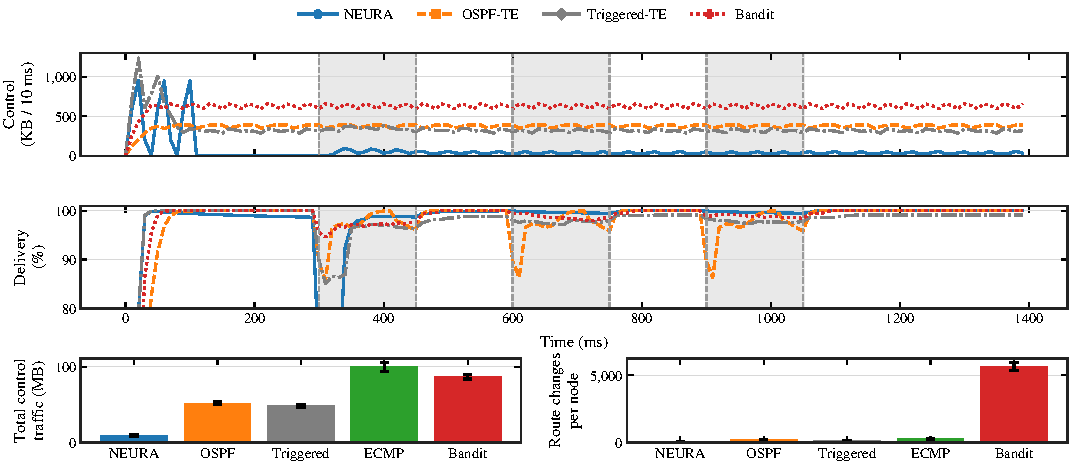
\includegraphics[width=\textwidth]{figures/generated/fig5_continuous_chaos.pdf}
\caption{Continuous-chaos behavior under three repeated hotspot shocks. The shaded intervals mark the disturbance windows. The upper panels show control traffic and delivery over time. The lower panels summarize cumulative control cost and route churn. NEURA keeps both totals far below the stronger baselines while preserving useful service.}
\label{fig:continuous-chaos}
\end{figure*}


\subsection{Safety and Packet-Level Validation}

The low-control operating point should not be interpreted as a relaxation of routing correctness. Table~\ref{tab:main-safety} reports compact safety indicators for the two main stress scenarios. NEURA returns to complete forwarding state in the tested runs and shows only low-amplitude transient loop activity during stress. The nearest triggered engineering baseline preserves strong service-window delivery, but it leaves a longer tail in the stricter all-destination table-completeness check.

\begin{table}[t]
\centering
\footnotesize
\caption{Compact post-startup safety indicators on ER-100. Reachability and loop values are worst cases over five seeds; final complete-route is the worst final node-complete-route ratio.}
\label{tab:main-safety}
\setlength{\tabcolsep}{3pt}
\begin{tabular}{llccc}
\toprule
Scenario & Method & \shortstack{Worst reach.\\(\%)} & \shortstack{Worst loop\\(\%)} & \shortstack{Final complete\\(\%)} \\
\midrule
Hotspot & NEURA & 99.87 & 0.13 & 100.0 \\
Hotspot & Triggered-TE & 98.97 & 1.03 & 6.0 \\
Repeated & NEURA & 99.87 & 0.13 & 100.0 \\
Repeated & Triggered-TE & 97.64 & 2.36 & 3.0 \\
\bottomrule
\end{tabular}
\end{table}

The ns-3 validation path then asks whether the same operating-point ordering remains visible when control and data are represented as packets, queues are DropTail device queues, and route decisions interact with packet-level loss and delay. Four checks are included: trace replay of simulator-generated control and data traffic, an online queue-signal sanity check using sampled DropTail occupancy, a TCP CUBIC goodput sanity check on the same two-path topology, and an online ER-24 packet-level validation across five seeds.
\begin{table}[t]
\centering
\scriptsize
\caption{ns-3 validation summary. Replay preserves NEURA's control-byte advantage under real packet headers and shared queues. Queue-signal and TCP checks show that stronger burst transport performance can be obtained, but only with substantially more route rewriting and tail switching.}
\label{tab:ns3-summary}
\setlength{\tabcolsep}{4pt}
\renewcommand{\arraystretch}{1.05}
\begin{tabular}{@{}llcccc@{}}
\toprule
Panel & Method & \shortstack[c]{Hotspot\\ctrl. (MB)} & \shortstack[c]{Hotspot\\del. (\%)} & \shortstack[c]{Repeated\\ctrl. (MB)} & \shortstack[c]{Repeated\\del. (\%)} \\
\midrule
\multicolumn{6}{l}{\textbf{A. Shared-queue replay}} \\
\cmidrule(lr){1-6}
A & NEURA & 0.35 & 99.70 & 0.35 & 99.25 \\
A & Triggered-TE & 1.63 & 99.96 & 1.63 & 99.89 \\
A & OSPF-TE & 1.65 & 99.81 & 1.65 & 99.53 \\
\midrule
Panel & Method & \shortstack[c]{Route\\changes} & \shortstack[c]{Tail\\switches} & \shortstack[c]{Primary-flow\\del. (\%)} & \shortstack[c]{Final\\path} \\
\midrule
\multicolumn{6}{l}{\textbf{B. Queue-signal sanity}} \\
\cmidrule(lr){1-6}
B & NEURA & 1 & 0 & 100.0 & b \\
B & Triggered-TE & 4 & 2 & 100.0 & a \\
B & OSPF-TE & 12 & 0 & 100.0 & a \\
\midrule
Panel & Method & \shortstack[c]{Burst TCP\\goodput (Mbps)} & \shortstack[c]{Route\\changes} & \shortstack[c]{Tail\\switches} & \shortstack[c]{CWND\\drops} \\
\midrule
\multicolumn{6}{l}{\textbf{C. TCP CUBIC sanity}} \\
\cmidrule(lr){1-6}
C & NEURA & 6.89 & 14 & 7 & 399 \\
C & Triggered-TE & 7.36 & 42 & 22 & 454 \\
C & OSPF-TE & 6.77 & 21 & 9 & 319 \\
\bottomrule
\end{tabular}
\end{table}
\begin{table}[t]
\centering
\scriptsize
\caption{Online ns-3 ER packet-level validation across five seeds. The controller samples real DropTail queue occupancy every $100$~ms on ER-24 packet-level topologies and rewrites source host routes online. This check is still not a full distributed protocol-stack implementation, but it exercises online packet-queue feedback beyond trace replay and the five-node sanity topology.}
\label{tab:ns3-online-er}
\setlength{\tabcolsep}{3.5pt}
\renewcommand{\arraystretch}{1.05}
\begin{tabular*}{\columnwidth}{@{\extracolsep{\fill}}llrrrr@{}}
\toprule
Scenario & Method & \shortstack[c]{Del.\\(\%)} & \shortstack[c]{Ctrl.\\(MB)} & \shortstack[c]{Route\\changes} & \shortstack[c]{Tail\\switches} \\
\midrule
Hotspot & NEURA & 97.9 & 0.003 & 10.6 & 0.6 \\
Hotspot & Triggered-TE & 98.3 & 0.007 & 21.6 & 11.6 \\
Hotspot & OSPF-TE & 99.9 & 0.885 & 29.2 & 12.0 \\
\midrule
Repeated & NEURA & 95.7 & 0.004 & 12.0 & 1.4 \\
Repeated & Triggered-TE & 96.6 & 0.014 & 43.2 & 23.2 \\
Repeated & OSPF-TE & 99.8 & 0.895 & 60.8 & 25.2 \\
\bottomrule
\end{tabular*}
\end{table}


Table~\ref{tab:ns3-summary} summarizes the replay, queue-signal, and TCP checks. In the replay panel, NEURA uses about $0.35$~MB of packetized control traffic in representative hotspot and repeated-disturbance replays, versus about $1.63$--$1.65$~MB for Triggered-TE and OSPF-TE, while delivery ratios remain tightly clustered near $100\%$. In the online queue-signal sanity check, all three methods preserve $100\%$ primary-flow delivery, but NEURA switches only once and exhibits no post-stress tail switch, whereas Triggered-TE switches four times and OSPF-TE rewrites the source route twelve times. The TCP CUBIC sanity check gives the same transport-facing picture: Triggered-TE recovers slightly higher burst goodput than NEURA, but with roughly three times as many route changes, more than three times as many tail switches, and more congestion-window drop events.

Table~\ref{tab:ns3-online-er} extends this external validation to ER-24 packet-level topologies. In the hotspot case, NEURA reaches $97.9\%$ delivery with about $0.003$~MB of ns-3 control transmission, compared with $98.3\%$ and $0.007$~MB for Triggered-TE, and $99.9\%$ and $0.885$~MB for OSPF-TE. Under repeated disturbance, NEURA reaches $95.7\%$ delivery with about $0.004$~MB of ns-3 control transmission and $1.4$ post-stress tail switches, while Triggered-TE reaches $96.6\%$ delivery with $0.014$~MB and $23.2$ tail switches, and OSPF-TE reaches $99.8\%$ delivery with $0.895$~MB and $25.2$ tail switches. The packet-level evidence therefore preserves the main ordering: engineering baselines can preserve somewhat stronger service, but NEURA keeps online route rewrites and packetized control burden much lower.
Because the ns-3 validation uses smaller packet-level topologies, different time windows, and packetized source-route rewrites, its byte totals are interpreted within each validation path rather than matched numerically to the ER-100 logical-control matrix. The mechanism-attribution and sensitivity studies in the supplementary material further separate the roles of memory, switch suppression, and parameter choices.

\subsection{Summary of Tradeoffs}
Overall, the results identify NEURA as a low-amplification routing-control operating point. It exhibits pressure-driven activation, a tightly localized blast radius, useful delivery under strong hotspot stress, and stable behavior under repeated disturbances. Triggered-TE shows that event-driven engineering is already a strong way to reduce unnecessary recomputation, while NEURA further changes the adaptation dynamics through memory, refractory suppression, and guarded recovery. The ns-3 online ER validation supports the same ordering under packetized control transmission and online DropTail queue feedback: NEURA maintains high delivery while using much less control traffic and producing far fewer tail switches.


\section{Discussion}

The evaluation positions NEURA as a routing-control operating point optimized for low amplification under stress. Periodic, multipath, and learning-based baselines often preserve higher burst-window delivery, but with substantially higher cumulative control traffic or route churn. Triggered-TE sharpens the comparison by showing that thresholded event-driven engineering is already a strong form of adaptation control. NEURA adds a local excitable structure in which accumulation, suppression, memory, and guarded recovery jointly bound the spatial and temporal expression of control activity.

The nearest-neighbor baseline also clarifies the role of the full mechanism. Memory and guarded switching mainly shape recovery behavior: they suppress rebound, reduce post-stress tail switching, and make repeated local route changes less attractive during recovery. This matters because route changes in a deployed router imply forwarding-table rewrites, cache effects, and local control work beyond simple message bytes. The control-byte accounting used here focuses on routing-law payloads, while implementation cost is analyzed through update and churn behavior. The combined traffic-and-churn picture shows how a local excitable law creates a different adaptation profile, especially for battery-powered and compute-limited stress-adaptive settings.

The most natural deployment context is resource-constrained, intermittently connected, emergency, tactical, or edge networking, where control links are expensive, local disturbances recur, and global reoptimization is too costly to invoke for every transient stress episode. In well-provisioned backbones whose primary objective is maximum throughput, strict shortest-path policy, or strong global consistency, conventional TE, ECMP, or learning-assisted optimization remains the more natural design point.

The evidence has a clear scope. The main evidence path is simulation-based, the topology families are stylized, and most service results are packet-delivery measurements under offered load. The baseline set covers periodic engineering, triggered engineering, multipath engineering, and lightweight online adaptation, while the ns-3 replay, queue-signal, TCP, and online ER checks add packet-level validation. These checks complement the routing simulator with packetized transmission, online queue feedback, and transport-facing measurements. For the distance-vector-like route-quality exchange used by NEURA, loop and blackhole behavior is reported through safety indicators under the tested workloads, while the formal analysis focuses on update-rate bounding and perturbation attenuation. Within this scope, the central result is consistent: localized routing-control laws can substantially reduce control activity and churn under severe local stress.

The broader implication is architectural. Routing adaptation can be shaped as an explicit local excitable process rather than only as repeated path recomputation or aggressive event triggering. A natural next step is to examine whether these mechanisms can be embedded more directly into switch-local agents, programmable data-plane assists, or lightweight network-control abstractions for self-healing communication fabrics.

\section{Conclusion}
This paper studied routing-control amplification under localized network stress and introduced NEURA as a local excitable routing-control law for stress-adaptive communication systems. NEURA combines local integration, threshold-triggered sparse updates, refractory suppression, short-term memory, and guarded switching to reduce control traffic and route churn under severe local stress.

The experimental evidence positions NEURA as a distinct low-amplification operating point. Relative to periodic, event-triggered, multipath, and learning-based baselines, it uses less control traffic and fewer forwarding-state rewrites in the tested hotspot and repeated-disturbance workloads while preserving useful delivery. Packet-level ns-3 validation supports the same reading under UDP/IP packets, DropTail queues, online queue sampling, and source-route rewrites.

The main implication is that severe local stress does not have to force proportionally large network-wide control activity when the routing law is localized, thresholded, suppressive, and recovery-aware. The results suggest that local excitable control is a useful protocol-construction principle for low-overhead self-healing communication systems, with a clear service-overhead tradeoff that is attractive for resource-constrained networks.

\section*{Data and Code Availability}
The simulation code, ns-3 validation programs, generated figure inputs, and result-audit outputs are available in the public reproduction repository at \url{https://github.com/unicorners-compin/neura-routing-artifact}. The internal code identifier \texttt{snn\_sra} is a development codename for NEURA and does not denote a separate method.

\section*{Funding}
This work was supported by the National Key Research and Development Program of China (No. 2024YFE0200300). The funder had no role in the study design, simulation design, data analysis, manuscript preparation, or decision to submit the article for publication.

\section*{Declaration of generative AI and AI-assisted technologies in the manuscript preparation process}
During the preparation of this manuscript, the authors used AI-assisted tools for language polishing, organization, and consistency checks. The tools were not used to generate scientific claims, conduct simulations, analyze data, or create figures. The authors reviewed and edited all content and take full responsibility for the final article.
\bibliographystyle{elsarticle-num}
\bibliography{refs/references}

\end{document}
